%% fichier sys_dig.tex
%%%%%%%%%%%%%%%%

\documentclass[a4paper, 12pt, twoside]{report}

\usepackage[utf8]{inputenc}
\usepackage[T1]{fontenc}
\usepackage[francais]{babel}
\usepackage{eurosym}
\usepackage{graphicx}
\usepackage{wrapfig}
\usepackage[bookmarks=true, bookmarksnumbered=true, linkcolor={0 0 1}, linkbordercolor={1 1 1}, pdfborderstyle={/S/U/W 1}]{hyperref}
\setcounter{tocdepth}{5}

\makeatletter
\renewcommand{\thesection}{\@arabic\c@section}
\makeatother

\usepackage{fancyhdr}
\usepackage{amsthm}
\usepackage{amsmath}
\usepackage{amsfonts}
\usepackage{amssymb}
\usepackage{mathrsfs}

\usepackage{enumerate}

\usepackage{color}
\definecolor{mygreen}{rgb}{0,0.6,0}
\definecolor{mygray}{rgb}{0.5,0.5,0.5}
\definecolor{mymauve}{rgb}{0.58,0,0.82}

\usepackage{listings}
\lstset{ %
  backgroundcolor=\color{white},   % choose the background color; you must add \usepackage{color} or \usepackage{xcolor}
  basicstyle=\footnotesize,        % the size of the fonts that are used for the code
  breakatwhitespace=false,         % sets if automatic breaks should only happen at whitespace
  breaklines=true,                 % sets automatic line breaking
  captionpos=b,                    % sets the caption-position to bottom
  commentstyle=\color{mygreen},    % comment style
  extendedchars=true,              % lets you use non-ASCII characters; for 8-bits encodings only, does not work with UTF-8
  frame=single,                    % adds a frame around the code
  keepspaces=true,                 % keeps spaces in text, useful for keeping indentation of code (possibly needs columns=flexible)
  keywordstyle=\color{blue},       % keyword style
  language=C,                 % the language of the code
  numbers=left,                    % where to put the line-numbers; possible values are (none, left, right)
  numbersep=5pt,                   % how far the line-numbers are from the code
  numberstyle=\tiny\color{mygray}, % the style that is used for the line-numbers
  rulecolor=\color{black},         % if not set, the frame-color may be changed on line-breaks within not-black text (e.g. comments (green here))
  showspaces=false,                % show spaces everywhere adding particular underscores; it overrides 'showstringspaces'
  showstringspaces=false,          % underline spaces within strings only
  showtabs=false,                  % show tabs within strings adding particular underscores
  stepnumber=1,                    % the step between two line-numbers. If it's 1, each line will be numbered
  stringstyle=\color{mymauve},     % string literal style
  tabsize=2,                       % sets default tabsize to 2 spaces
  title=\lstname                   % show the filename of files included with \lstinputlisting; also try caption instead of title
}


\usepackage[top=3cm, bottom=3cm, left=3cm, right=3cm]{geometry}

\lhead{Ecole Normale Supérieure}
\rhead{}
\lfoot{}
\rfoot{}
\renewcommand{\headrulewidth}{0.4pt}
\renewcommand{\footrulewidth}{0.4pt}

\newcommand{\HRule}{\rule{\linewidth}{0.5mm}}
\pagestyle{fancy}

\newtheorem{definition}{Définition}[section]
\newtheorem{proposition}{Proposition}[section]

\begin{document}
%%%%%%%%%%%%%%%%

\begin{titlepage}
\begin{center}

% Upper part of the page. The '~' is needed because \\
% only works if a paragraph has started.

\includegraphics[width=0.35\textwidth]{./ENS_Logo.png}~\\[1cm]

\textsc{\Large Système Digital}\\[0.5cm]

% Title
\HRule \\[0.4cm{ \huge \bfseries Microprocesseur \\[0.4cm] }
\large{\textit{Implémentation d'une horloge digitale}}]

\HRule \\[1.5cm]
\end{center}

% Author and supervisor
\begin{minipage}{0.4\textwidth}
\begin{flushleft} \large
\emph{Auteurs :}\\
Nicolas ASSOUAD\\
Rémi JEZEQUEL\\
Jules PONDARD\\
Hugo MANET\\
\end{flushleft}
\end{minipage}

\begin{center}
\vfill
% Bottom of the page
{\large \today}

\end{center}
\end{titlepage}

\newpage\strut
%%%%%%%%%%%%%%%%
\tableofcontents
\thispagestyle{fancyplain}

\newpage~
\newpage~
%%%%%%%%%%%%%%%%

\section*{Introduction}
\addcontentsline{toc}{section}{Introduction}

Dans le cadre du cours de Système Digital, nous sommes amenés à concevoir un microprocesseur
qui sera capable notamment d'exécuter un programme de montre électronique.
Nous allons d'abord présenter les choix de conception de notre microprocesseur
puis nous discuterons du programme de l'horloge digitale en lui même.

\newpage~
\newpage~

\section{Le Microprocesseur}

\subsection{Le concept}

Notre ligne directrice de conception de notre microprocesseur a été de n'implémenter que 
les opérations de bases en matériel, et de laisser le soin au programmeur ou à un 
éventuel compilateur de les combiner pour produire des opérations plus évoluées.
Néanmoins, le jeu d'instruction pourrait être encore plus réduit, mais cela ne jouerait 
pas en faveur des performances.\\

Notre Microprocesseur est une machine "little endian". Cela signifie que les nombres 
sont représentés en machine avec leur bits de poids faible en premier. Cela explique 
les codages qui vont suivre.\\

Le microprocesseur possède 32 registres différents dont certains spéciaux comme le 
pointeur d'instructions PC. Il sont numérotés de 1 à 32, le  $30^{ieme}$ registre étant 
le registre contenant l'overflow, le $31^{ieme}$ registre étant le 
registre contenant la valeur des "flag", et le $32^{ieme}$ registre étant lui le 
registre du compteur d'instructions. Ils sont codés sur 6 bits. La valeur du registre est codée 
sur les 5 premiers bits, et le $6^{ieme}$ bit permet de savoir si l'adressage est direct 
c'est à dire que c'est la valeur du registre qui est souhaitée (valeur 0), ou indirect 
c'est à dire que c'est la valeur se trouvant à l'adresse contenue dans le registre qui 
est souhaitée (valeur 1).\\

Les mots mémoires sont des mots de 32 bits, si bien que toutes les opérations matérielles
se font sur des entiers de 32 bits. Les nombres écrit en dur dans les instructions dites 
"immediate" sont eux codés sur 16 bits.\\


Nous allons présenter ici plus ou moins grossièrement le déroulement d'un cycle (pour une vision 
plus détaillée, il est préférable d'aller regarder directement le fichier Minijazz qui 
décrit notre microprocesseur) :

\begin{itemize}
\item Les valeurs des différents registres sont récupérées
\item L'instruction pointée par le pointeur d'instruction est chargée de la ROM
\item Une première selection s'opère, elle permet de déterminer si l'on est en 
      présence d'une instruction qui utilise des nombres "immediate" ou pas, ou 
      d'une instruction utilisant des registres à adressage en mémoire indirecte.
      Dans le cas de l'utilisation d'une instruction "immediate", le nombre codé 
      sur 16 bits est alors étiré en un nombre de 32 bits en copiant sont dernier 
      bit. Cela permet de gérer les nombres "immediate" signés.
\item Tout les calculs possibles sont effectués par le microprocesseur, s'en suit 
      alors une seconde sélection qui détermine par rapport au code de l'instruction 
      le résultat voulu. (Voir schéma)
\item On met alors à jour les registres (avec un traitement spécial pour les registres 
      de pointeur d'instruction, de "flag", et de "overflow").\\
\end{itemize}

\begin{figure}[!h]
\centering
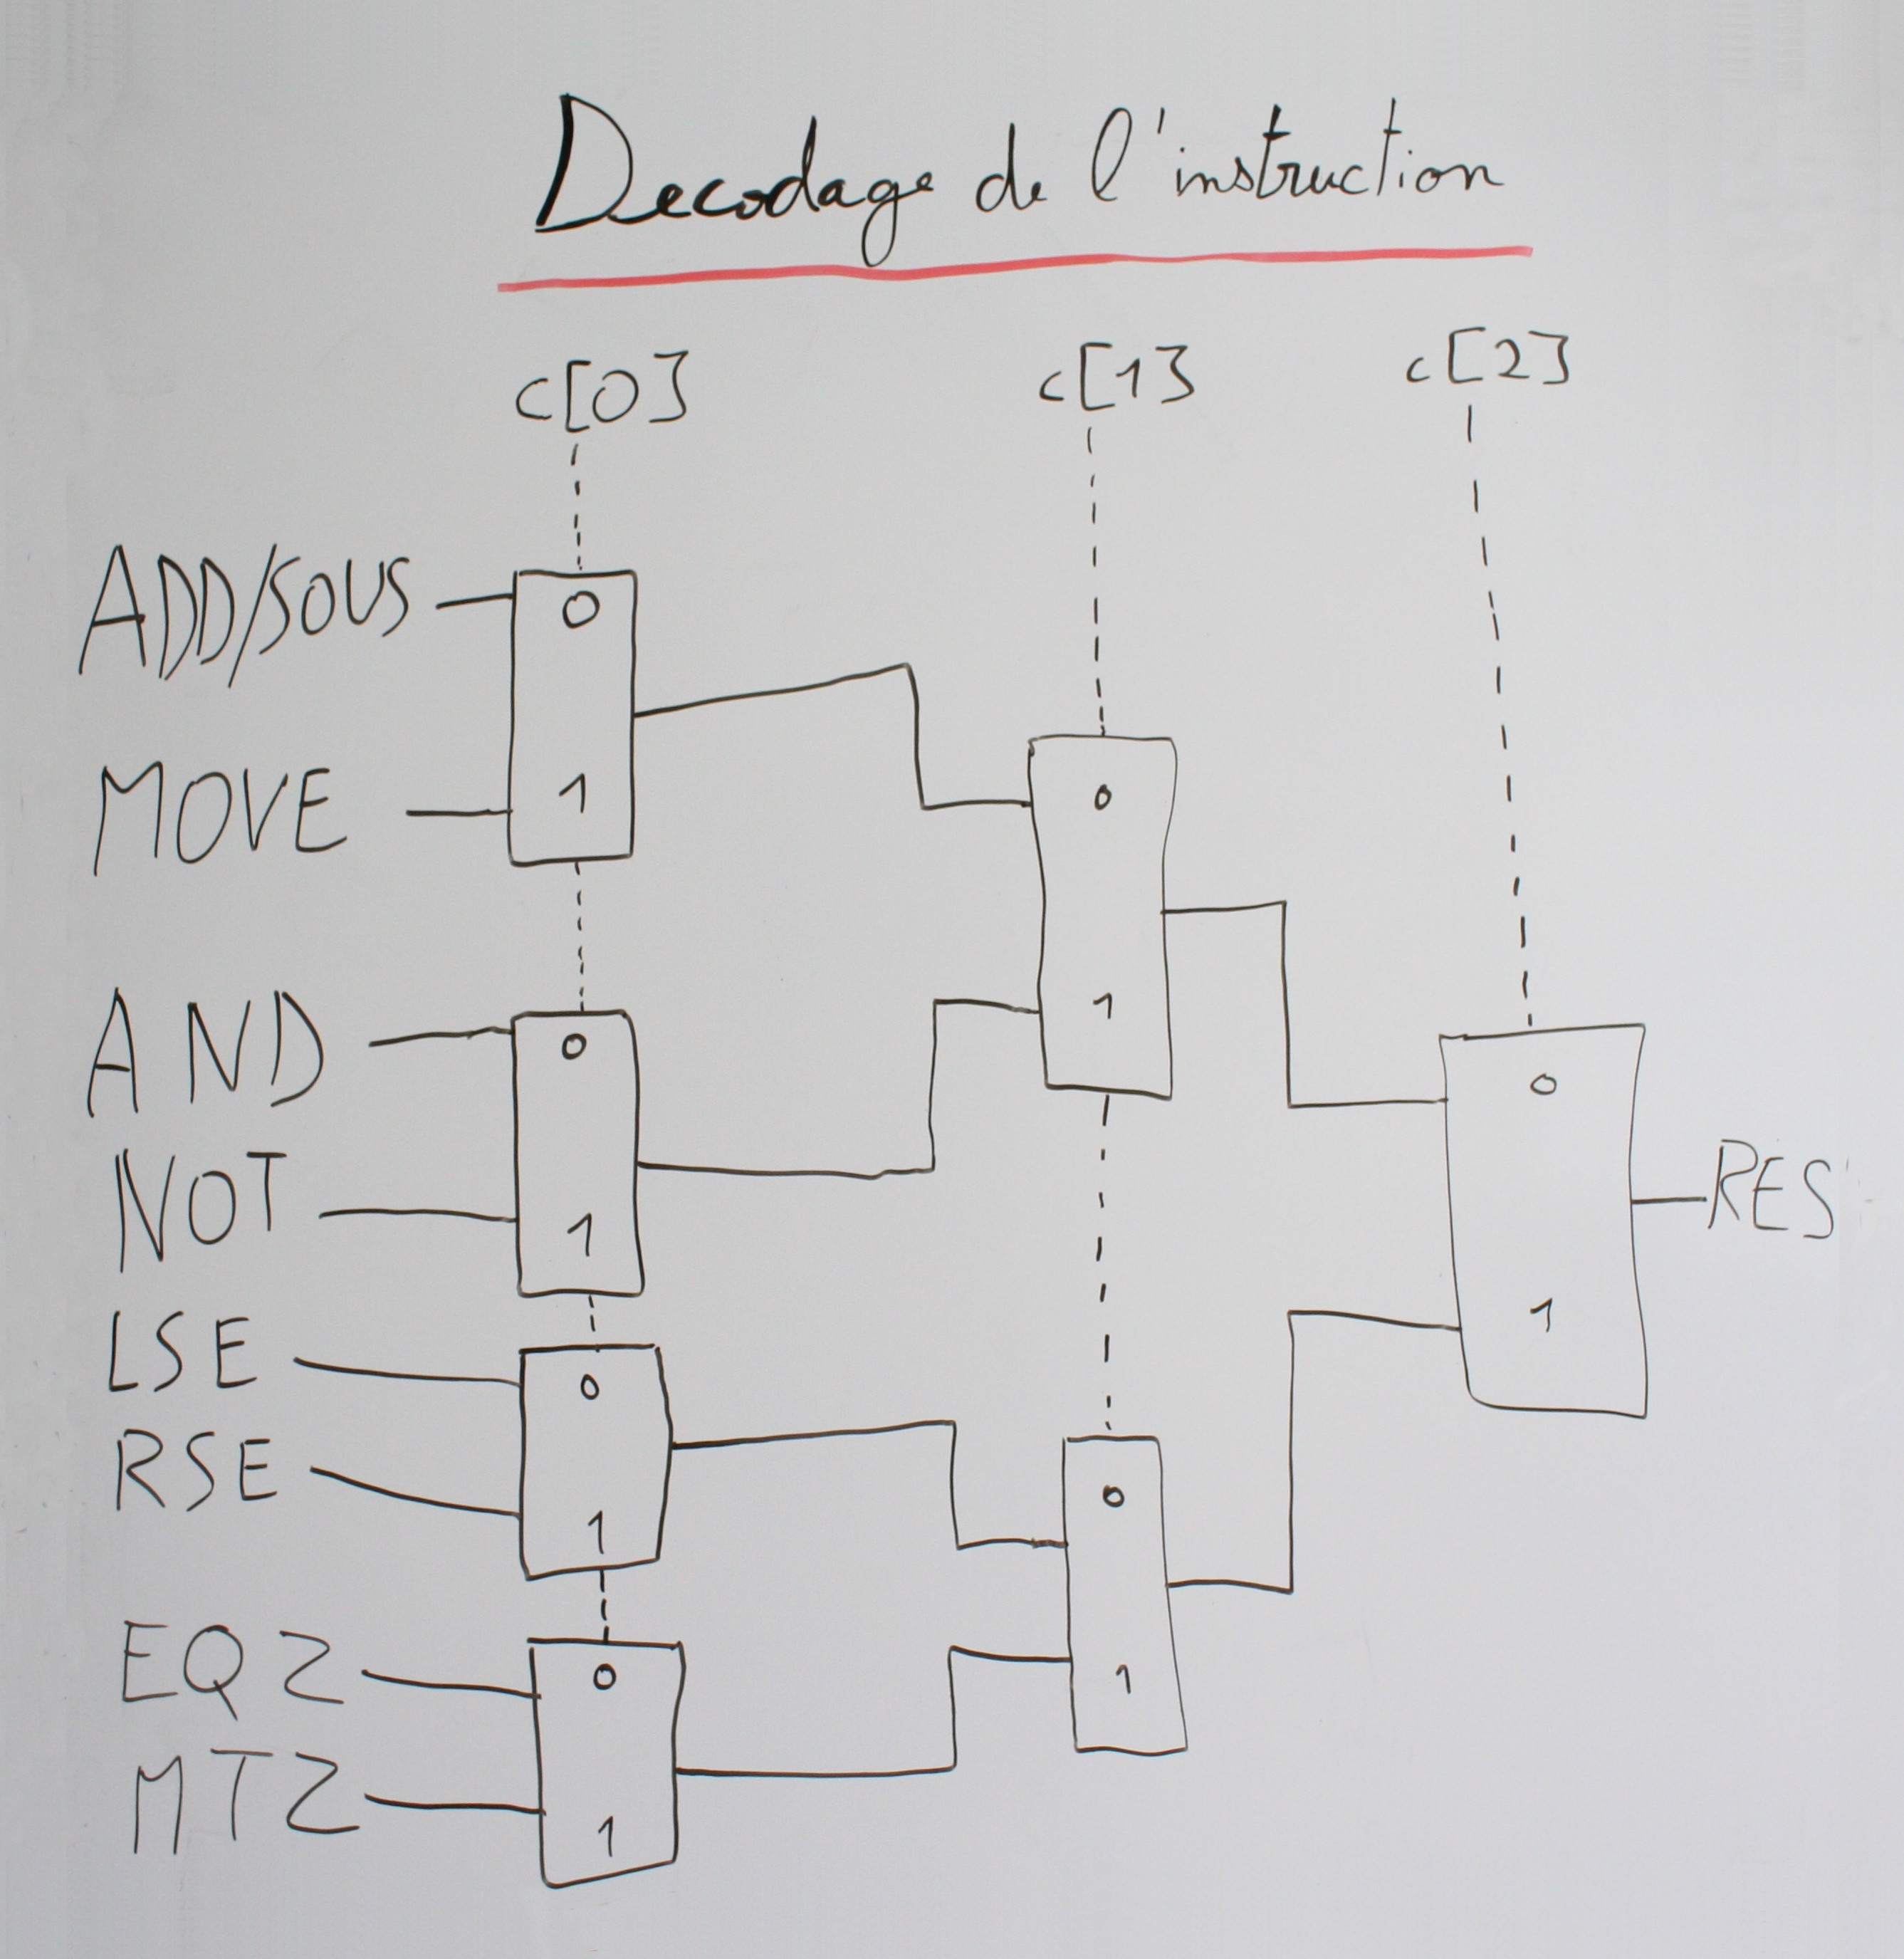
\includegraphics[width=10cm]{tabnic.jpg}
%\caption{Cryptage Asymétrique}
\end{figure}

\subsection{Les instructions matérielles}

Les instructions du microprocesseur sont codées sur 27 bits. Les 4 premiers bits 
codent l'instruction voulue. Le reste du codage de l'instruction dépend de sa nature.
Si la description du codage d'une instruction ne va pas jusqu'à 27 bits (notamment
quand il n'y a pas d'argument entier), il est sous entendu que le code de 
l'instruction est complété par des zéros à la fin.\\

Le codage d'une instruction implique toujours deux opérandes, même si c'est une 
instruction qui ne prends qu'un seul argument. Cette représentation redondante permet 
de simplifier les processus de sélection de cible du résultat d'une instruction dans 
l'architecture du microprocesseur, et cela n'est en rien une perte, car de toute façon 
les instructions sont codées sur 27 bits, autant en utiliser le maximum lorsque cela est utile.\\

Le microprocesseur supporte les 12 instructions suivantes.\\

\subsubsection{ADD(i)}

L'instruction ADD implémente l'addition. Elle s'emploie de la façon suivante :
ADD a b. Cette instruction calcule la somme des valeurs contenues dans les mémoires
a et b, et place le résultat dans la mémoire b.\\
L'instruction supporte que sont premier paramètre soit directement un nombre, l'addition
s'effectue alors directement avec celui-ci.\\

Le code de l'instruction prend la forme suivante :

\begin{tabular}{|c|c|c|c|c|}
  \hline
  0000 & 0 & premier registre (a) & second registre (b) & 0000000000 \\
  \hline
\end{tabular}\\

Dans le cas ou le premier argument est directement un entier (instruction ADDi),
le code de l'instruction prend cette forme :

\begin{tabular}{|c|c|c|c|}
  \hline
  0000 & 1 & entier (sur 16 bits) & registre (b) \\
  \hline
\end{tabular}\\

\subsubsection{SUB(i)}

L'instruction SUB implémente la soustraction. Elle s'emploie de la façon suivante :
SUB a b. Cette instruction calcule la différence des valeurs contenues dans les mémoires
a et b (b - a), et place le résultat dans la mémoire b.\\
L'instruction supporte que sont premier paramètre soit directement un nombre, la soustraction
s'effectue alors directement avec celui-ci.\\

Le code de l'instruction prend la forme suivante :

\begin{tabular}{|c|c|c|c|c|}
  \hline
  0001 & 0 & premier registre (a) & second registre (b) & 0000000000 \\
  \hline
\end{tabular}\\

Dans le cas ou le premier argument est directement un entier (instruction SUBi),
le code de l'instruction prend cette forme :

\begin{tabular}{|c|c|c|c|}
  \hline
  0001 & 1 & entier (sur 16 bits) & registre (b) \\
  \hline
\end{tabular}\\

\subsubsection{MOVE(i)}

L'instruction MOVE implémente la copie d'octet. Elle s'emploie de la façon suivante :
MOVE a b. Cette instruction déplace le contenu de la mémoire a vers la mémoire b. 
L'instruction supporte que sont premier paramètre soit directement un nombre, c'est alors 
directement celui-ci qui est envoyé vers la mémoire b.\\

Le code de l'instruction prend la forme suivante :

\begin{tabular}{|c|c|c|c|c|}
  \hline
  1000 & 0 & premier registre (a) & second registre (b) & 0000000000 \\
  \hline
\end{tabular}\\

Dans le cas ou le premier argument est directement un entier (instruction MOVEi),
le code de l'instruction prend cette forme :

\begin{tabular}{|c|c|c|c|}
  \hline
  1000 & 1 & entier (sur 16 bits) & registre (b) \\
  \hline
\end{tabular}\\


\subsubsection{AND}

L'instruction AND implémente un "et" logique bit à bit. Elle s'emploie de la façon suivante :
ADD a b. Cette instruction calcule le "et" logique entre les bits de la mémoire de a et b, 
et place le résultat dans la mémoire b.\\

Le code de l'instruction prend la forme suivante :

\begin{tabular}{|c|c|c|c|c|}
  \hline
  0100 & 0 & premier registre (a) & second registre (b) & 0000000000 \\
  \hline
\end{tabular}\\

\subsubsection{NOT}

L'instruction NOT implémente un "non" logique bit à bit. Elle s'emploie de la façon suivante :
NOT a. Cette instruction calcule le "non" logique des bits de la mémoire de a,
et place le résultat dans la mémoire a.\\

Le code de l'instruction prend la forme suivante :

\begin{tabular}{|c|c|c|c|c|}
  \hline
  1100 & 0 & registre (a) & registre (a) & 0000000000  \\
  \hline
\end{tabular}\\

\subsubsection{LSE}

L'instruction LSE implémente un décalage de un bit à gauche (donc une multiplication par deux). 
Elle s'emploie de la façon suivante : LSE a. Cette instruction décale les bits à gauche de la mémoire 
de a, et place le résultat dans la mémoire a.\\

Le code de l'instruction prend la forme suivante :

\begin{tabular}{|c|c|c|c|c|}
  \hline
  0010 & 0 & registre (a) & registre (a) & 0000000000 \\
  \hline
\end{tabular}\\

\subsubsection{RSE}

L'instruction RSE implémente un décalage de un bit à droite (donc une division par deux). 
Elle s'emploie de la façon suivante : RSE a. Cette instruction décale les bits de la mémoire 
à droite de a, et place le résultat dans la mémoire a.\\

Le code de l'instruction prend la forme suivante :

\begin{tabular}{|c|c|c|c|c|}
  \hline
  1010 & 0 & registre (a) & registre (a) & 0000000000 \\
  \hline
\end{tabular}\\

\subsubsection{EQZ(i)}

L'instruction EQZ implémente un saut conditionnel si le flag indique une égalité à zéro. 
Elle s'emploie de la façon suivante : EQZ a. Si le flag indique une égalité à zéro, 
cette instruction incrémente le pointeur d'instruction de la valeur contenue dans 
la mémoire a.\\
L'instruction supporte que sont premier paramètre soit directement un nombre, la saut
s'effectue alors directement avec celui-ci. Le registre cyble est le registre du pointeur 
d'instruction. C'est le registre numéro 32, il a donc comme code 111110 (adressage direct).\\

Le code de l'instruction prend la forme suivante :

\begin{tabular}{|c|c|c|c|c|}
  \hline
  0110 & 0 & registre (a) & 111110 & 0000000000 \\
  \hline
\end{tabular}\\

Dans le cas ou le premier argument est directement un entier (instruction EQZi),
le code de l'instruction prend cette forme :

\begin{tabular}{|c|c|c|c|}
  \hline
  0110 & 1 & entier (sur 16 bits) & 111110 \\
  \hline
\end{tabular}\\

\subsubsection{MTZ(i)}

L'instruction MTZ implémente un saut conditionnel si le flag indique une supériorité à zéro. 
Elle s'emploie de la façon suivante : MTZ a. Si le flag indique une supériorité à zéro, 
cette instruction incrémente le pointeur d'instruction de la valeur contenue dans 
la mémoire a.\\
L'instruction supporte que sont premier paramètre soit directement un nombre, la saut
s'effectue alors directement avec celui-ci. Le registre cyble est le registre du pointeur 
d'instruction. C'est le registre numéro 32, il a donc comme code 111110 (adressage direct).\\

Le code de l'instruction prend la forme suivante :

\begin{tabular}{|c|c|c|c|c|}
  \hline
  1110 & 0 & registre (a) & 111110 & 0000000000 \\
  \hline
\end{tabular}\\

Dans le cas ou le premier argument est directement un entier (instruction MTZi),
le code de l'instruction prend cette forme :

\begin{tabular}{|c|c|c|c|}
  \hline
  1010 & 1 & entier (sur 16 bits) & 111110 \\
  \hline
\end{tabular}\\

\newpage~
\newpage~


\section{Le Simulateur}

\subsection{Présentation}

Nous allons présenter ici le travail réalisé dans le cadre de la conception du simulateur 
de NETLIST. Dans sa version final (contrairement au rendu intermédiaire), il n'a plus 
la vocation de simuler n'importe quel circuit, mais il est orienté plus particulièrement 
vers notre microprocesseur.\\

Les NETLIST sont des fichiers qui décrivent un circuit électronique synchrone par 
l'intermédiare de ses équations. Les fonctionnalités a implémentées sont notamment 
toutes les opérations logiques, la prise en compte des registres, la prise en 
compte des nappes de fils, ainsi que la mise en place de primitives mémoire RAM et 
ROM.\\

Notre simulateur de NETLIST n'est pas un interpréteur, mais un compilateur. Il va 
compiler des NETLIST en un fichier source écrit en langage C. Ce fichier source 
sera alors un programme qui implémentera le circuit compilé, si bien qu'une fois 
transformé en langage machine par l'intermédiaire d'un compilateur C, nous serons 
en possession d'un exécutable qui sera capable de simuler notre NETLIST.\\

L'utilisation de ce simulateur se fait en trois étapes :
\begin{itemize}
\item Tout d'abord, le fichier NETLIST est compilé vers du C. Il faut prendre bien soin de 
      fournir au compilateur les noms des fichiers qui contiendront le contenu de la ROM et 
      de la RAM en début de simulation
\item Puis le fichier source C est compilé via un compilateur C comme gcc
\item On lance le programme crée qui peut alors simuler le circuit décrit par la NETLIST initiale\\
\end{itemize}

Notre simulateur ne suit pas à la lettre les spécifications du sujet, en effet, ses arguments 
se limitent au seul nombre de cycles demandé au simulateur. Le choix de ne pas fournir d'entrées 
à notre simulateur vient du fait que notre microprocesseur ne demande pas d'entrées pour fonctionner.\\

Les commandes de compilation sont précisées dans le fichier LISEZ\_MOI du projet.\\

\subsection{Détails d'implémentation}
Nous allons discuter ici des choix d'implémentations de notre simulateur. 
Tout d'abord, toute les données utilisées par notre simulateur se trouvent sous la forme 
d'une suite de 0 ou de 1 ASCII dans des fichiers. Les nombres doivent notamment être représentés 
avec leur bits de poids faible en premier ("little endian") pour respecter la politique de notre microprocesseur. 
Cela concerne les fichiers d'initialisation de la ROM et de la RAM.\\

Si l'on regarde plus précisément ce qu'il se passe dans le cas de notre microprocesseur, 
la ROM contient le code à exécuter, et la RAM est initialisée avec des valeurs utiles. La structure de 
la RAM pour notre microprocesseur est la suivante :
\begin{itemize}
\item l'adresse 0 contient le nombre de secondes écoulées depuis que le microprocesseur est en marche
\item l'adresse 1 est l'adresse d'affichage des secondes
\item l'adresse 2 est l'adresse d'affichage des minutes
\item l'adresse 3 est l'adresse d'affichage des heures
\item l'adresse 4 est l'adresse d'affichage des jours
\item l'adresse 5 est l'adresse d'affichage des années
\item de l'adresse 6 à 10 se trouvent des constantes utilisées par le programme de l'horloge
\item à partir de l'adresse 11 se trouvent des "lookup table".\\
\end{itemize}

Les adresses 1, 2, 3, 4, 5 sont les adresses d'affichages. Le contenu de ces cases mémoires sont 
affichés tout les cycles.\\

Dans le fichier C généré, la RAM et la ROM sont chargées en mémoire intégralement. Au cours 
des différents cycles, l'accès à la mémoire est donc direct.\\


Chaque variable de la NETLIST donne lieu à une variable dans le fichier C généré. On 
observe ces différents cas :
\begin{itemize}
\item les nappes de fils de taille n sont représentées par un tableau statique de char de taille n
\item les RAM et les ROM sont représentées par des tableaux de tableaux alloués dynamiquement. Prenons le cas 
      de notre microprocesseur 32 bits. Les adresses de la RAM ou de la ROM sont en toute logique 
      codé sur des nombres en 32 bits, et les cases mémoires contiennent des nombres de 32 bits qui 
      sont donc représentés par des tableaux de taille 32. Pour que le simulateur fonctionne correctement, 
      on ne lui demande pas d'allouer un tableau dynamique de taille $2^{32}$ pour représenter toute la 
      mémoire, on suppose que la mémoire utile est donnée dans les fichiers d'initialisations. La taille 
      de la mémoire allouée est donc la taille des fichiers d'initialisations.
\item les variables de type bit sont représentées par de simples variables de type char\\
\end{itemize}

Les équations sont traduites en langage C de manière quasi direct, avec l'utilisation de fonction 
simples dans le cas de commande sur les nappes de fils. Elles suivent l'ordre donné par le tri 
topologique appliqué au graphe des équations lors de la compilation. Les variables qui 
apparaissent comme argument d'une fonction REG dans la NETLIST sont traité d'une manière particulière. 
Pour qu'elles soient mis à jour convenablement et donc qu'elles remplissent correctement leurs 
rôle de registre, leur équations qui leur donne leur valeur sont placées à la toutes fin d'un 
cycle. Elles peuvent ainsi être représentées par une seule variable malgré leur status de registre.

\newpage~
\newpage~

\section{Le programme de l'horloge}

\subsection{Notre assembleur}
Notre microprocesseur met en place un certain nombre d'instructions. Pour ne pas avoir 
à les traduire nous même en une suite de 0 et 1, nous avons implémenté un assembleur 
qui automatisera cette tâche. En plus d'automatiser cette tâche, notre assembleur va 
mettre en place un système de macro qui va rendre plus aisé l'écriture de programme.\\

La structure de nos fichier source et la suivantes : une suite de définition de macros 
entre les balises \#MACRO et \#ENDMACRO, puis les instructions du programme principal. 
Il ne faut pas voir les macros comme des étiquettes auxquelles on accède par des sauts, 
elles ne sont la que pour faciliter la lecture et la compréhension du code et s'apparentent 
plus au préprocesseur du langage C.\\

\subsection{Le code de l'horloge}

Pour programmer le programme de l'horloge, nous avons du réaliser différentes fonctions.
Tout d'abord, il fallait réaliser des fonctions de calcul de modulo. Pour une horloge, les 
modulos intéressants sont les modulos 60, 24 et 365. Nous sommes d'abord partis 
sur l'idée de faire des modulos de petits nombres premiers : 3, 5, 73, et de les combiner (les 
modulos d'une puissance de 2 étant facilement optenus avec un masque). Cette approche fut 
abandonnée, en effet, cela aurait entrainé l'implémentation d'un algorithme des restes chinois 
qui aurait été trop lourd à exécuter.\\

Les modulos sont donc réalisés directement. Pour cela, on utilise une technique qui s'apparente à
celle vu en cours. Prenons le cas de 60. Nous traitons des entiers de 32 bits. On remarque que 
$2^{16} \text{ mod } 60 = 16$, nous allons donc additionnner la partie haute multipliée par 16 
et la partie basse de cette entier 32 bits. En répétant l'opération 3 fois, on constate que le 
résultat tiens forcément sur 16 bits. On a donc réduit le problème au calcul du modulo 60 d'un 
nombre 16 bits. On réutilise la même méthode de découpe, et il s'avère que là aussi on a :
$2^{8} \text{ mod } 60 = 16$. On arrive alors à un nombre sur 8 bits. Le calcul du modulo 60 d'un 
nombre sur 8 bits se fait en recherchant sa valeur dans une table se trouvant en RAM dans laquelle 
est stockée les différentes valeurs du modulo pour un octet. On obtient donc la macro suivante 
pour le calcul du modulo 60 :\\
\begin{lstlisting}
MOD60(X) {
    // On effectue le calcul trois fois car 2^16 mod 60 = 16,
  MOVE X, R10;
  MOVEi 10, R13; // Recuperation du masque FFFF en memoire.
  MOVE *R13, R13;
  AND R13, R10;
  MOVEi 16, R11;
  RS R11, X;
  // 2^16 mod 24
  LSE X;
  LSE X;
  LSE X;
  LSE X;
  ADD R10, X;
  MOVE X, R10;
  AND R13, R10;
  MOVEi 16, R11;
  RS R11, X;
  // 2^16 mod 24
  LSE X;
  LSE X;
  LSE X;
  LSE X;
  ADD R10, X;
  MOVE X, R10;
  AND R13, R10;
  MOVEi 16, R11;
  RS R11, X;
  // 2^16 mod 24
  LSE X;
  LSE X;
  LSE X;
  LSE X;
  ADD R10, X;
  
    // Par le calcul quatre etapes
  MOVE X, R10;
  MOVEi 255, R13;
  AND R13, R10;
  MOVEi 8, R11;
  RS R11, X;
  // 2^8 mod 24
  LSE X;
  LSE X;
  LSE X;
  LSE X;
  ADD R10, X;
  MOVE X, R10;
  AND R13, R10;
  MOVEi 8, R11;
  RS R11, X;
  // 2^8 mod 24
  LSE X;
  LSE X;
  LSE X;
  LSE X;
  ADD R10, X;
  MOVE X, R10;
  AND R13, R10;
  MOVEi 8, R11;
  RS R11, X;
  // 2^8 mod 24
  LSE X;
  LSE X;
  LSE X;
  LSE X;
  ADD R10, X;
  
  ADDi 267, X; // Calcul de l'adresse dans la lookup table du modulo 60 (sur 1 octet et non pas sur 4 bits)
  MOVE *X, X;
}
\end{lstlisting}

Nous avons aussi implémenté un algorithme de multiplication. C'est une multiplication 
egyptienne à nombre d'instructions constant. Il calcule la multiplication de deux nombres de
32 bits, le résultat est stocké sur un nombre de 64 bits, sa partie basse étant placée dans 
le registre R1 et sa partie haute étant placée dans le registre R2.\\

\begin{lstlisting}
MUL(X1, X2) {
  MOVEi 0, R1;
  MOVEi 0, R2;
  MOVEi 1, R29;
  MOVEi 32, R23;
  MOVE X2, R26; // Partie Basse
  MOVEi 0, R27; 
  MOVE X1, R22;
  AND R29, R22; // Recuperation du premier bit
  MOVEi 0, R28;
  SUB R22, R28; // MASQUE
  MOVE R26, R25;
  AND R28, R25;
  ADD R25, R1;
  ADD R30, R2;
  MOVE R27, R25;
  AND R28, R25;
  ADD R25, R2; // ADDITION SI NECESSAIRE
  MOVE R26, R25;
  MOVEi 31, R24;
  RS R24, R25;
  LSE R26;
  LSE R27;
  ADD R25, R27;
  RSE X1;
  SUBi 1, R23;
  MTZi -21;
}
\end{lstlisting}

Les divisions par une constante sont réalisées par l'algoritheme de Barrett. 
Il consiste à calculer une constante "magique", puis à multiplier celle si à notre nombre, et enfin 
effectuer un décalage à celui-ci pour trouver le quotient. Reprenons notre exemple de 60. 
En pratique, si l'on souhaite diviser des nombres de 32 bits divisible par 60 par 60, on calcule 
la constante magique $x = \frac{2^{32}}{60}$ et l'on multiplie $x$ et notre nombre. On décale ensuite 
vers la droite 32 fois (c'est à dire on divise par $2^{32}$). Comme notre algorithme de multiplication 
nous renvoie déjà un nombre coupé en deux mots de 32 bits, il suffit de prendre la partie haute pour avoir 
le nombre décalé. Cela nous donne le code suivant, toujours pour 60 :\\
\begin{lstlisting}
DIV60(X) {
  MOVEi 7, R10;
  MOVE *R10, R10;
  MUL R10, X;
  MOVE R2, X;
}
\end{lstlisting}

Le programme de l'horloge final consiste juste à récupérer le nombre de seconde écoulées depuis 
le début du programme, et à effectuer le différents modulos et divisions pour calculer le nombre 
de secondes, de minutes, d'heures, de jours et d'années.

\newpage~

\section*{Conclusion}
La réalisation d'un processeur est une tâche difficile. Il faut trouver le bon compromis 
entre une architecture efficace et pas trop complexe et un jeu d'instructions suffisament 
évolué pour une programmation aisée. L'autre défi de celui-ci est la simulation. 
Contrairement au monde physique où les différents éléments d'un cycle se calculeraient quasiment 
en parallèle, le simulation ne peut le réaliser que séquentiellement ce qui n'est pas en faveur de 
bonnes performances.

\addcontentsline{toc}{section}{Conclusion}

\end{document}


